\section{Error Ellipses and Ellipsoids}
Given the point $(X,Y)$:
\begin{align*}
X &= 10 \pm 2 \\
Y &= 20 \pm 4 \\
\end{align*}


Error ellipses(2D) and ellipsoids(3D) are used to depict the region in which a point is expected to lie within a percentage of the time.  The percentage of the time the point is expected to lie within the region indicates the confidence.  For example, a 1\% confidence region is much smaller than a 99\% confidence region, as shown in the figure below. In other words, based on the uncertainty in the measurement, the true value will only lie within the 1\% error ellipse 1\% of the time.  The center of an error ellipse is the \textit{most probable value}.
\[
\Sigma = 
\begin{bmatrix}
\sigma_X^2 & \sigma_{XY} \\
\sigma_{XY} & \sigma_Y^2 
\end{bmatrix}
=
\begin{bmatrix}
4 & 3 \\
3 & 10 
\end{bmatrix}
\]
\begin{figure}[H]
	\centering
	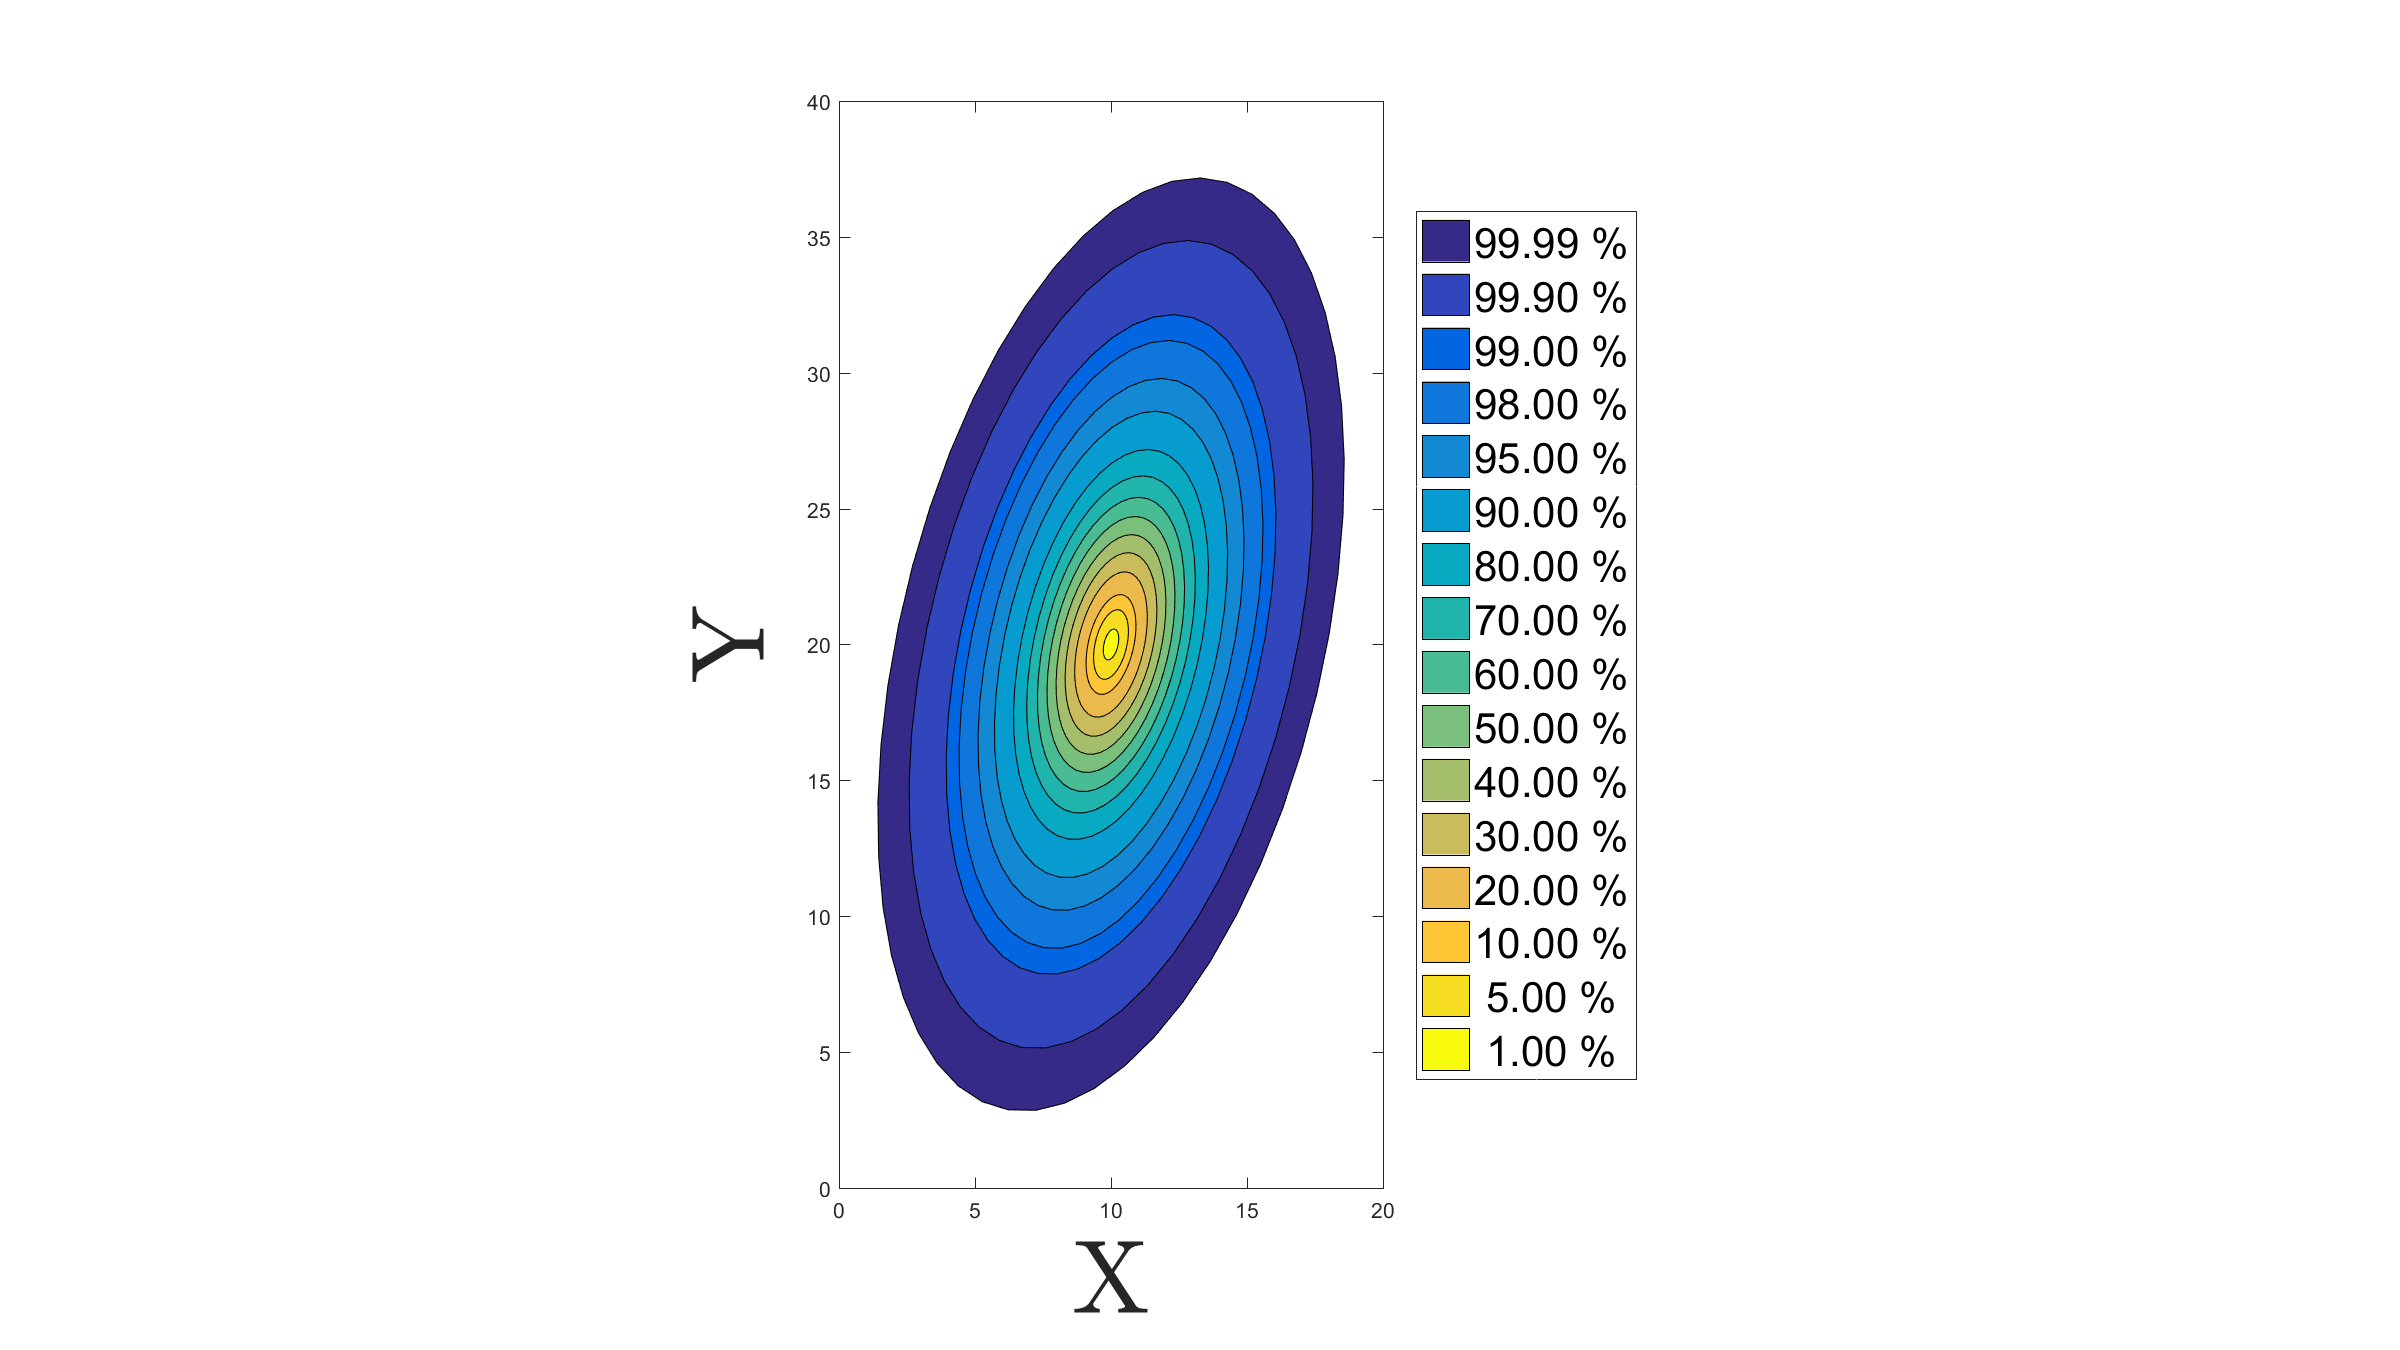
\includegraphics[height = 4in]{ellipsefig.png}
\end{figure}

Note that the \textit{Standard Error Rectangle} is a rectangle centered on the most probable value, with a width of $2\sigma_X$ and a height of $2\sigma_Y$.  It is another way to depict the expected region in which a value lies.  

\subsection{Calculation of Semi-Major and Semi-Minor Axes}
\todo{need to add this section}